%
% Einleitung
%

\chapter{Programm}

\section{Aufbau}
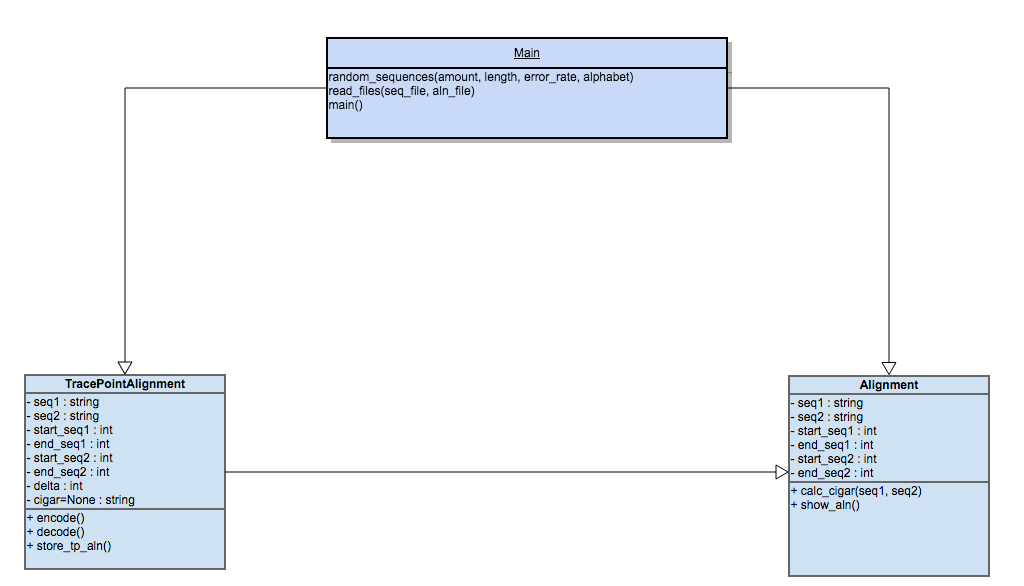
\includegraphics[width=\textwidth]{images/UML}
\section{Funktionalit�t}
\subsection{Informationsverlust bei 'encode()'}
Die encode-Funktion extrahiert aus dem gegebenen CIGAR-String die Trace Points, welche dann zusammen mit dem $\Delta$-Wert und den Start- und Endpositionen der Sequenzabschnitte gespeichert werden. Hierbei geht die Information, wie die jeweiligen Intervalle zwischen den Trace Points zu den komplement�ren Intervallen in der Ursprungssequenz aligniert werden, verloren.
F�r die R�ckgewinnung dieser Information muss in der 'decode()'-Funktion zun�chst ein neues Alignment der jeweiligen Intervall-Paare errechnet werden.

\section{Grafiken Geschwindigkeit, Speicher}